\documentclass[a4paper,titlepage,openright,12pt]{report}
\usepackage{graphicx}    
%\usepackage{epsfig}   
\usepackage[font=footnotesize]{subfig}
\usepackage{float}
\usepackage{fancyhdr}                              
\usepackage{makeidx}
\usepackage[nottoc,notlot,notlof]{tocbibind}     
\usepackage{supertabular}
\usepackage{array}              
\usepackage{setspace} 
\usepackage{enumerate}
\usepackage{rotating}
\usepackage{moreverb}
\usepackage{multirow}
\usepackage{amsmath}
\usepackage{amsthm}
\usepackage{amssymb}
\usepackage{captcont}
\usepackage{verbatim}
\usepackage{titlesec}
\usepackage{url}
\usepackage{hyperref}
\usepackage{lipsum}
\usepackage{listings}
\usepackage{color}

\definecolor{dkgreen}{rgb}{0,0.6,0}
\definecolor{gray}{rgb}{0.5,0.5,0.5}
\definecolor{mauve}{rgb}{0.58,0,0.82}

\lstset{frame=tb,
  language=Java,
  aboveskip=3mm,
  belowskip=3mm,
  showstringspaces=false,
  columns=flexible,
  basicstyle={\small\ttfamily},
  numbers=none,
  numberstyle=\tiny\color{gray},
  keywordstyle=\color{blue},
  commentstyle=\color{dkgreen},
  stringstyle=\color{mauve},
  breaklines=true,
  breakatwhitespace=true,
  tabsize=3
}
%\usepackage[algoruled]{algorithm2e}
%\usepackage[figure,algoruled]{algorithm2e}
%\usepackage[figure,boxruled]{algorithm2e}

%\newtheorem{theorem}{Theorem}
%\newtheorem{corollary}[theorem]{Corollary}
%\newtheorem{conjecture}[theorem]{Conjecture}
%\newtheorem{lemma}[theorem]{Lemma}
%\newtheorem{proposition}[theorem]{Proposition}
%\newtheorem{definition}[theorem]{Definition}
%\newtheorem{Example}[theorem]{Example}
%\newtheorem{axiom}{Axiom}
%\newtheorem{remark}{Remark}
%\newtheorem{exercise}{Exercise}[section]
%\newtheorem{fact}[theorem]{Fact}
%\newtheorem{property}[theorem]{Property}
\setlength{\parindent}{0pt}%for paragraph spacing
\setlength{\parskip}{1ex plus 0.5ex minus 0.2ex}
\setlength{\textheight}{8.5in}
\pagestyle{fancy}
% with this we ensure that the chapter and section
% headings are in lowercase.
%\renewcommand{\bibname}{References}
\renewcommand{\chaptermark}[1]{\markboth{#1}{}}
\renewcommand{\sectionmark}[1]{\markright{\thesection\ #1}}
\fancyhf{} % delete current setting for header and footer
\fancyhead[LE,RO]{\bfseries\thepage}
\fancyhead[LO]{\bfseries\rightmark}
\fancyhead[RE]{\bfseries\leftmark}
%\rfoot{\bfseries\thepage}
\cfoot{\em $\copyright$ 2013, Indian Institute of Technology Delhi}
\renewcommand{\headrulewidth}{0.5pt}
\renewcommand{\footrulewidth}{0.5pt}
\addtolength{\headheight}{2.5pt} % make space for the rule

\fancypagestyle{plain}{%
\fancyhead{} % get rid of headers on plain pages
\fancyfoot{}
%\rfoot{\bfseries\thepage}
\cfoot{\em $\copyright$ 2015, Indian Institute of Technology Delhi}
\renewcommand{\headrulewidth}{0pt} % and the line
}

%% The smart version of cleardouble page.
\let\origdoublepage\cleardoublepage
\newcommand{\clearemptydoublepage}{%
  \clearpage
  {\pagestyle{empty}\origdoublepage}%
}

\let\cleardoublepage\clearemptydoublepage


\date{}


\addtolength{\oddsidemargin}{30pt}
\addtolength{\evensidemargin}{-40pt}

\titlespacing*{\chapter}{0pt}{-50pt}{20pt}
\titleformat{\chapter}[display]{\normalfont\huge\bfseries}{\chaptertitlename\ \thechapter}{20pt}{\Huge}
% \DeclareGraphicsExtensions{.pdf,.png,.jpg,.ps}
\floatstyle{boxed} 
\restylefloat{figure}
\setcounter{lofdepth}{2}
\setcounter{lotdepth}{2}

\newtheorem{claim}{Claim}[section]
\newtheorem{theorem}{Theorem}[section]
\newtheorem{defn}{Definition}[section]
\newtheorem{fact}{Fact}[section]

\graphicspath{{./Figures/}}
\begin{document}

%\begin{comment}
% Begin title page
\begin{titlepage}
\begin{center}

\LARGE{\textsf{\bfseries Energy Management System}}\\
\vspace{20pt}
\normalsize
\emph{A thesis submitted in partial fulfillment} \\
\emph{of the requirements for the degree of} \\
\vspace{20pt}
\bfseries BACHELOR OF TECHNOLOGY \\
\vspace{20pt}
\emph {in}\\
\vspace{20pt}
\bfseries Electrical Engineering (Power and Automation) \\
\vspace{20pt}
\emph {by}\\
\vspace{20pt}
\begin{center}
\begin{tabular}{ c c }
 \Large{\textsf{\bfseries Pranav Verma}} & \Large{\textsf{\bfseries 2015EE30528}} \\ 
\Large{\textsf{\bfseries N. Akash }} & \Large{\textsf{\bfseries 2015EE30522}} \\
\end{tabular}
\end{center}

\ \\
%\ \\
{\normalsize \emph {Under the guidance of}}
\ \\
\Large{\textsf{\bfseries Prof. B K Panigrahi}} \\
\ \\
\vspace{30pt}
%\begin{center}

\includegraphics[scale=0.2]{iit_logo.pdf} \\
\vspace{10pt}
%\end{center}
\large{\textsc{Department of Electrical Engineering,\\
Indian Institute of Technology Delhi.\\ November 2018.}}
\end{center}
\end{titlepage}
%\newpage
%\cleardoublepage
\onehalfspacing
\thispagestyle{empty}

\normalfont
\begin{center}
\LARGE{ Certificate} 
\end{center}

\vspace{0.5in}

This is to certify that the thesis titled {\bfseries Energy Management System} being submitted by
{\bfseries Pranav Verma and N. Akash} for the award of {\bfseries Bachelor of Technology} in {\bfseries Electrical Engineering (Power and Automation)} is a record of bona fide work carried out by them under my guidance and supervision at the {\bfseries Department of Electrical Engineering}. The work presented in this thesis has not been submitted elsewhere either in part or full, for the award of any other degree or diploma.

\vspace{1.5in}


{\bfseries B K Panigrahi} \\
{\bfseries Department of Electrical Engineering} \\
{\bfseries Indian Institute of Technology, Delhi}\\ 

\thispagestyle{empty}
%\begin{center}
\LARGE{Acknowledgments} 
\end{center}

\vspace{0.5in}

%Replace \lipsum with your acknowledgement
\lipsum[1]

\vspace{1.5in}

{\bfseries Pranav Verma,} \\
{\bfseries N. Akash}

\thispagestyle{empty}


% \setcounter{page}{1}
% \pagenumbering{roman}
\thispagestyle{empty}
\begin{center}
\LARGE{Abstract}
\end{center}

\vspace{0.5in}

%replace \lipsum with your abstract
With increasing complexities in electrical grids as well as increasing demand for power, it is pertinent that the grid is safely and efficiently maintained. This can be done using an end to end system which can perform an Observability Analysis and State Estimation based on the grid data. This can enable engineers to make better decisions. Such a system has been implemented in a modular, easy to use python package. 



\thispagestyle{empty}
\begin{center}
\LARGE{Acknowledgments} 
\end{center}

\vspace{0.5in}

%Replace \lipsum with your acknowledgement
\lipsum[1]

\vspace{1.5in}

{\bfseries Pranav Verma,} \\
{\bfseries N. Akash}


\thispagestyle{empty}
\tableofcontents

\thispagestyle{empty}

\listoffigures

\listoftables
%\end{comment}

\thispagestyle{empty}
\cleardoublepage
\onehalfspacing
%%%%%%%%%%%%%%%%%%%%%%%%%%%%%%%%%%%%%%%%%%%%%%%%%%%%%%%%%%%%
 
\setcounter{page}{1}
\pagenumbering{arabic}

%You may have as many chapters as you please. This is just for reference.   

\chapter{Introduction}

%Replace \lipsum with text.
% You may have as many sections as you please. This is just for reference.

\section{SECTION NAME}
\lipsum[1]

You should cite papers in the following manner: Bayliss et al.~\cite{Bay1} gave an iterative method for Helmholtz equation etc.
Similar work has been done in \cite{Bailey,Ernst,Gold3}.

% You may add figures in the following manner.
\begin{figure}[h]
\begin{center}	
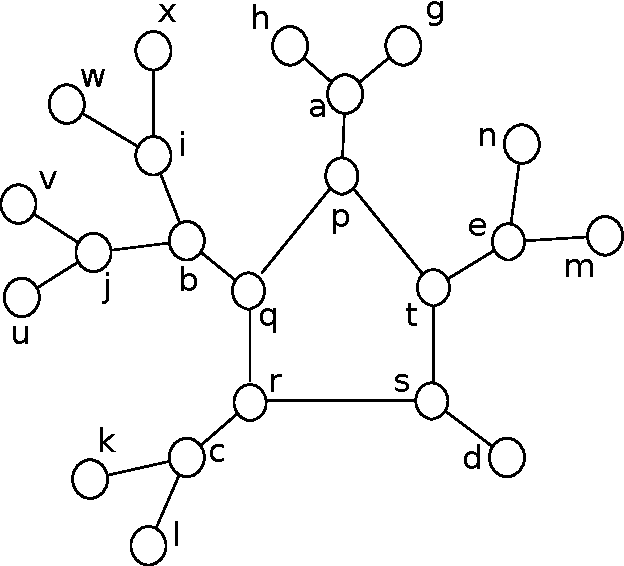
\includegraphics[scale=0.4]{pent} 
\caption{Pentagon $pqrst$}
\label{fig:pent}
\end{center}
\end{figure}

\lipsum[1]

\section{SECTION NAME}
\lipsum[2]

\begin{table}
\centering
\begin{tabular}{| c | c |}
\hline
{\bf item 1} & {\bf item 2} \\ \hline
%
abcde & 5 \\ \hline
%
pqrst & 4 \\ \hline
\end{tabular}
\caption{A sample table}
\label{table:1}
\end{table}

\chapter{CHAPTER NAME}

%Replace \lipsum with text.
% You may have as many sections as you please. This is just for reference.

\section{SECTION NAME}
\lipsum[2]

\section{SECTION NAME}
\lipsum[3]

\section{SECTION NAME}
\lipsum[2]

\chapter{Setup}
In this chapter we explain the setting up of RTDS model and the code for observability analysis and state estimation

%Replace \lipsum with text.
% You may have as many sections as you please. This is just for reference.

\section{RTDS}
RTDS \cite{rtds} is a popular simulation hardware used to run real time power line simulations. It is commonly  used for studies of protective relays, control systems, power hardwares, etc. We use this hardware primarily to simulate a Transmission line and generate and record data for further analysis, such as observability analysis, state estimation, Optimum Power Flow, etc.\\
RSCAD is a simulation software that is used to create models of power lines, to work on the RTDS Simulator Hardware. For our project we set up a model for a 14 bus power line system, with specifications taken from IEEE 14 Bus power system \cite{IEEE14bus}. The model has the following characteristics:
\begin{itemize}
\item Number of Buses: 14
\item Number of Lines: 20
\item Number of Generators: 5
\end {itemize}
The overall system that we designed looked like Figure ~\ref{fig:ckt}.\\
\begin{figure}[h]
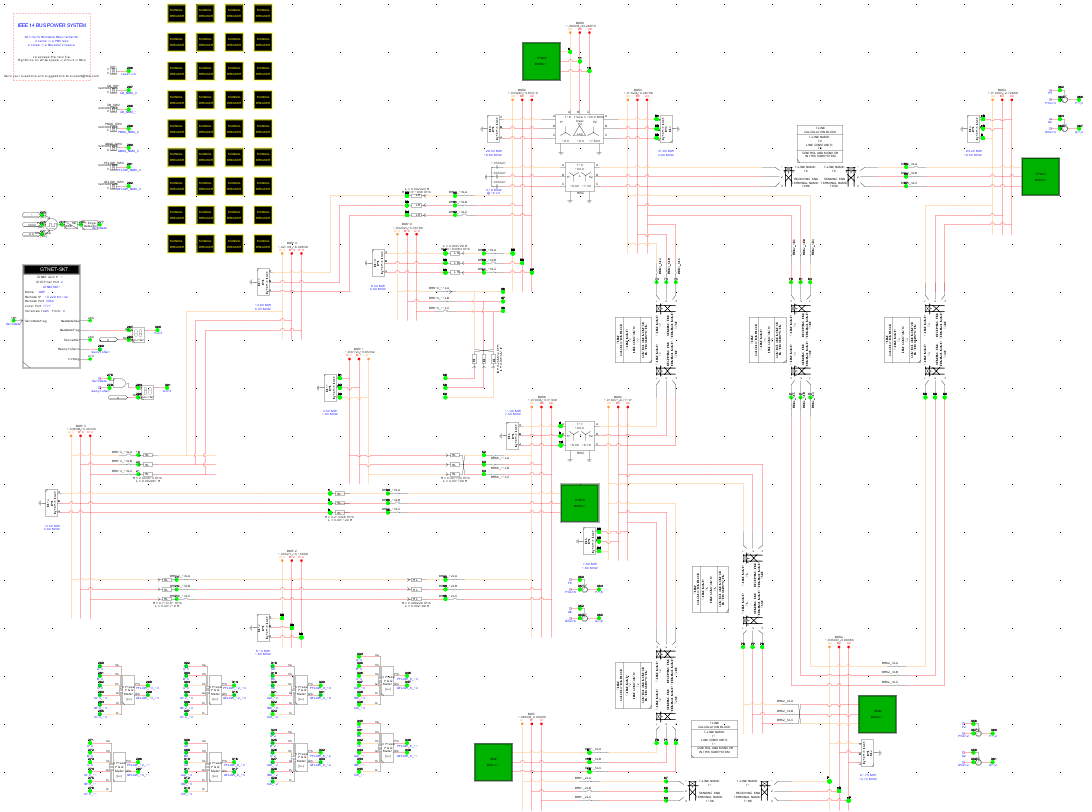
\includegraphics[width=\textwidth]{Figures/ckt.png}
\caption{IEEE 14 Bus Power Line System Model on RSCAD}\label{fig:ckt}
\end{figure}

It had the following key blocks, shown here for reference. (~\ref{fig:bus} to ~\ref{fig:skt})

\begin{figure}[h]
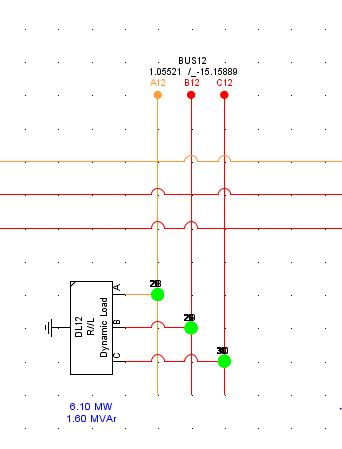
\includegraphics[width=\textwidth]{Figures/bus.jpg}
\caption{Typical Bus in RSCAD}\label{fig:bus}
\end{figure}

\begin{figure}[h]
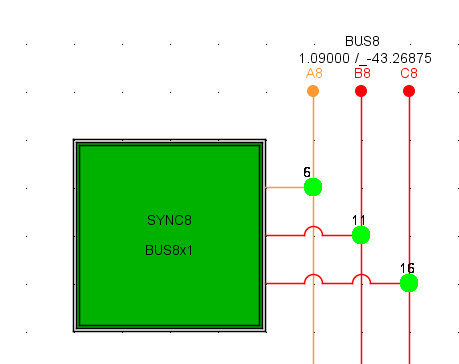
\includegraphics[width=\textwidth]{Figures/gen.png}
\caption{Generator Block in RSCAD}\label{fig:gen}
\end{figure}

\begin{figure}[h]
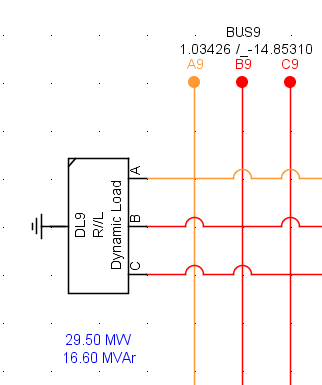
\includegraphics[width=\textwidth]{Figures/load.png}
\caption{PQ load Block in RSCAD}\label{fig:load}
\end{figure}

Apart from the main network, we have the GTNET-SKT block ( Figure ~\ref{fig:skt}), which is crucial for sending and receiving data from RTDS to our server, which records and processes data for further analysis of the power system.  To function, it needs the following parameters specified:
\begin{itemize}
\item All the signals to be measured. In our case, these were the status about all the circuit breakers in the system, the real and complex power injections, real and complex power flows in the lines, and status about availability of each measurement
\item The remote IP address and port of the server to which data is to be sent. 
\end{itemize}
GTNET-SKT 
To simulate real life situations where all data measurements are not available, we also toggle the availability of measurements recorded by GTNET-SKT. Furthermore, we calculate and transmit measurements we call \emph{status numbers}, which provide us information about which measurements are available, and which are not.
\begin{figure}[h]
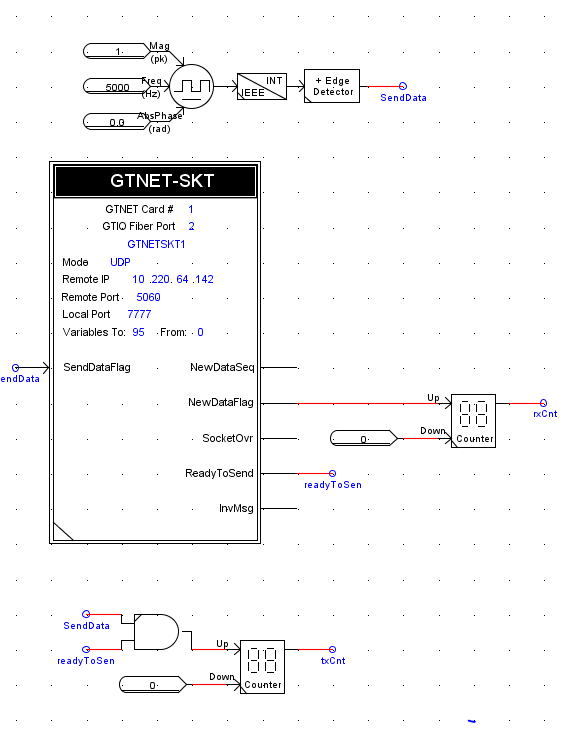
\includegraphics[width=\textwidth]{Figures/skt.png}
\caption{GTNET-SKT Block in RSCAD}\label{fig:skt}
\end{figure}



\section{SECTION NAME}
\lipsum[3]

\section{SECTION NAME}
\lipsum[2]

\chapter{Experimental Results}

%Replace \lipsum with text.
% You may have as many sections as you please. This is just for reference.

\section{Transfer of Data from RTDS to server}
\begin{figure}
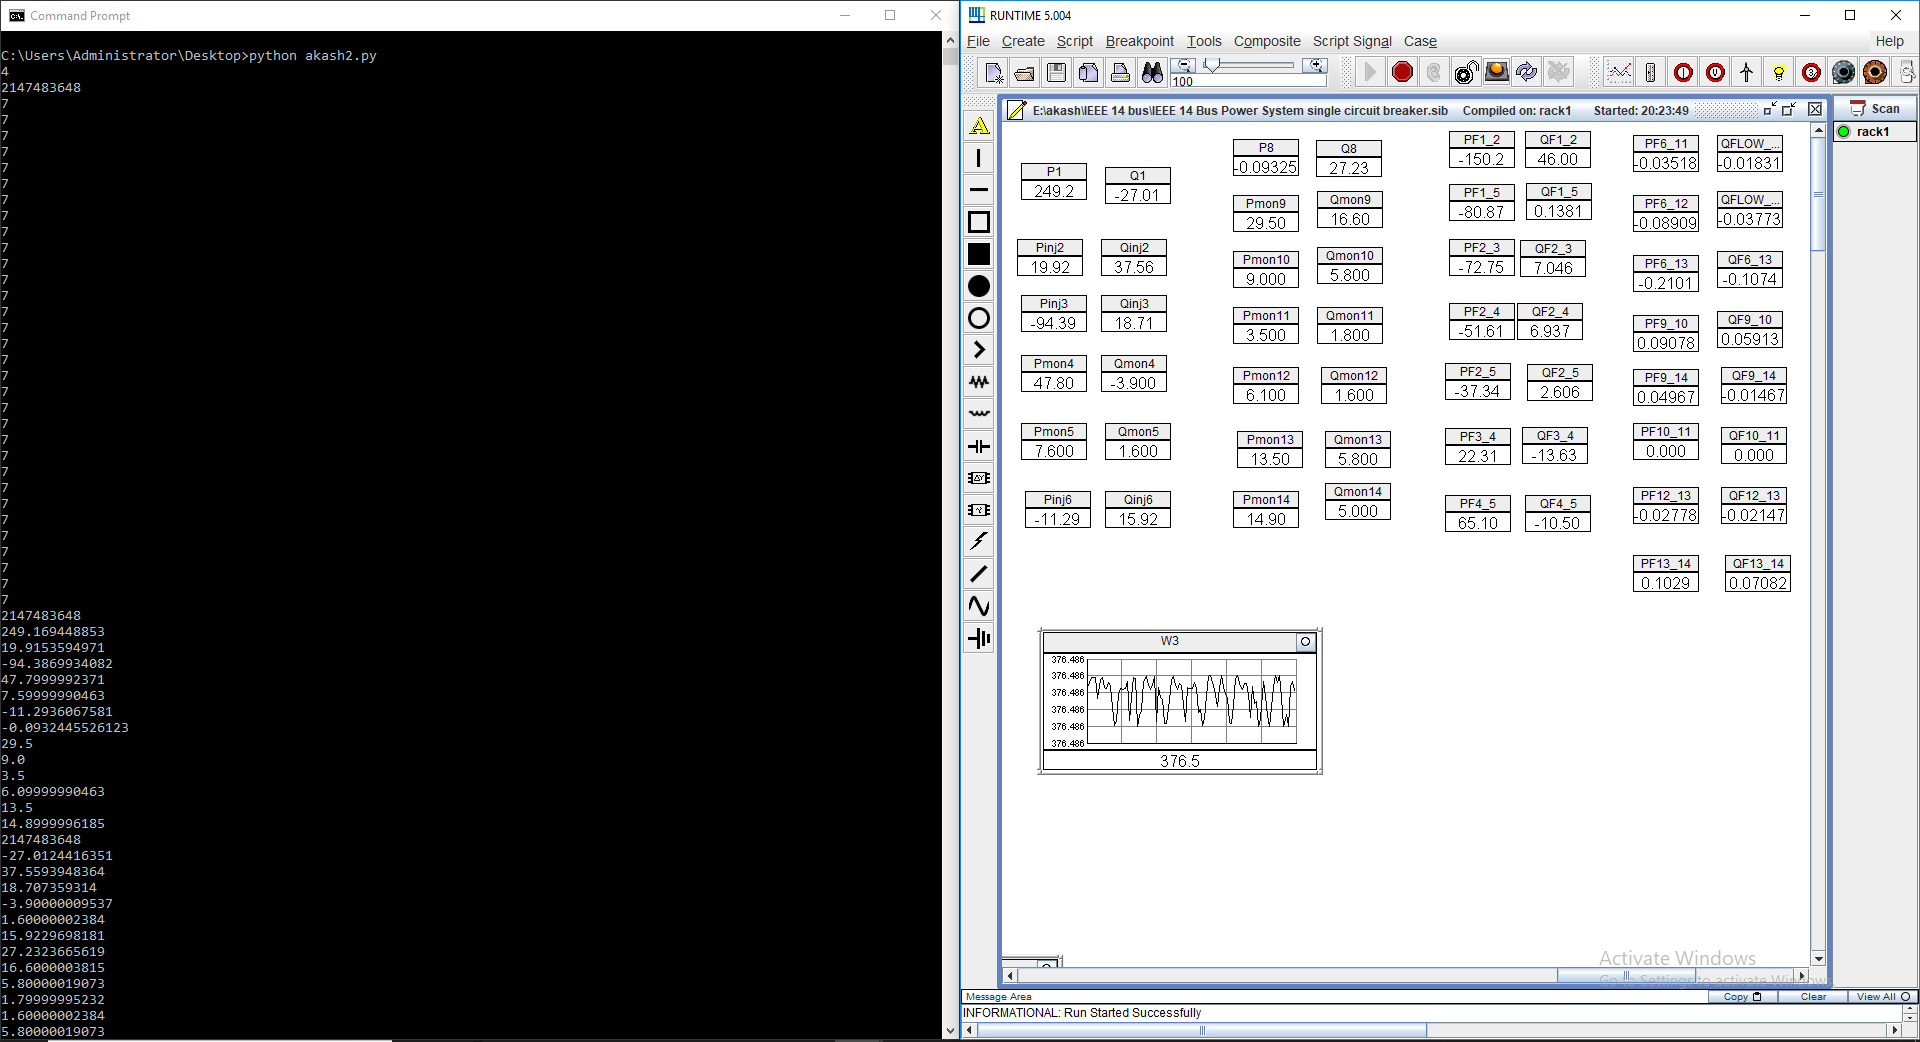
\includegraphics[width=\textwidth]{Figures/response_dt_cb.png}
\caption{Transfer of real and reactive power injections and flows from RTDS (right) to server (left), Observing circuit breaker status}
\label{fig:data_transfer_cb_status}
\end{figure}

\begin{figure}
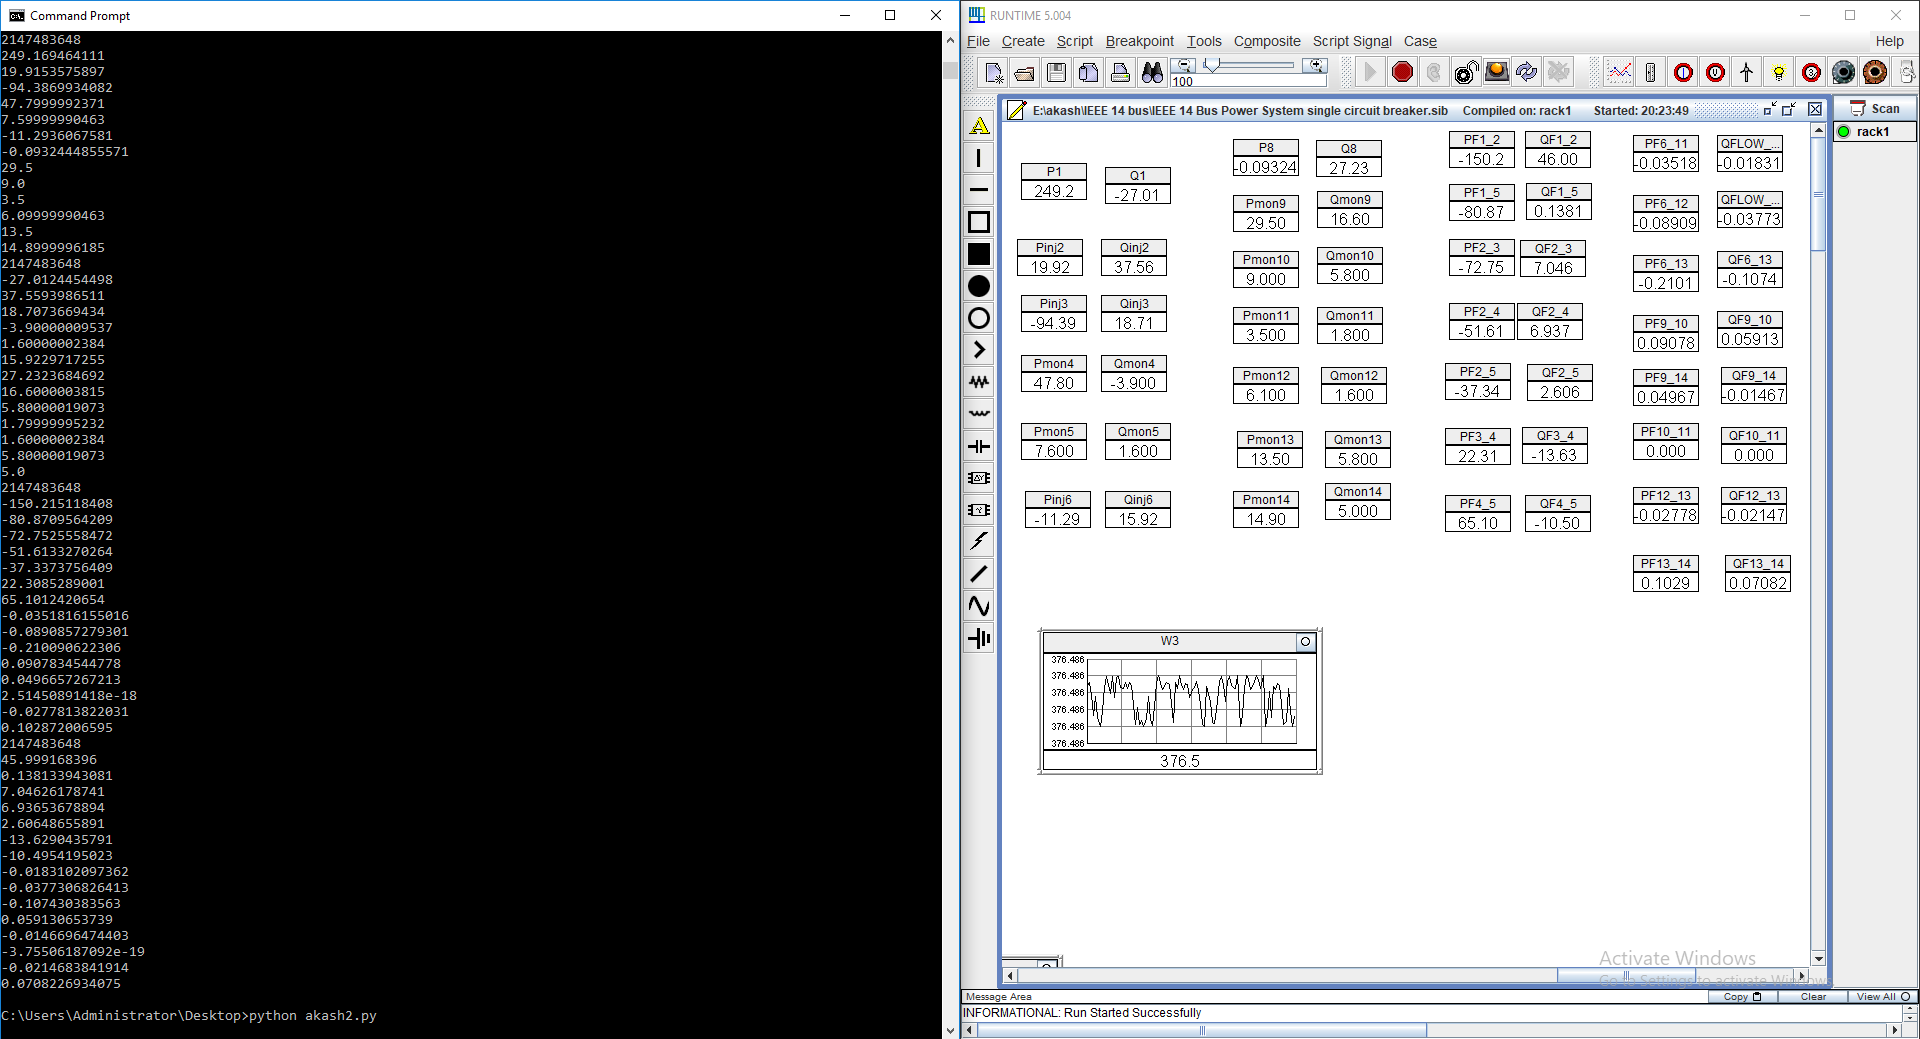
\includegraphics[width=\textwidth]{result_dt2.png}
\caption{Transfer of real and reactive power injections and flows from RTDS (right) to server (left)}
\label{fig:data_transfer}
\end{figure}

In Figure ~\ref{fig:data_transfer}, we observe real time data transfer from RTDS via GTNET-SKT to our server, which we built using a python script running on the Desktop. Here the measurements come in the order described in chapter 3 (Real injection then reactive . The value 4294967295 ($2^{32}-1$) is the status number for the set of measurements. All bits are 1, signifying all measurements are available. In Figure ~\ref{fig:data_transfer_cb_status}, we observe the availability status of all circuit breakers in the system. The first number is the case\_number, and 4 represents 14 bus system. Circuit breakers status number is also 4294967295, signifying all circuit breakers are available. Circuit breaker measurement of 7 represents all 3 phases are ON (3 bits are 1).\\
The graph is the frequency response curve of the system, in rad/s. The system operates at $376.5/2 \pi=60Hz$ with very little fluctuation.\\

This shows that we have been able to extract all the available measurements, and identify which measurement belongs to which variable, without using many extra measurement variables.

\section{Observability Analysis and State Estimation}
After collecting data, we perform observability analysis. If the system is found to be observable, we perform state estimation.
Here, for the above example, the system performs state estimation since all measurements are available. In fact, since all the measurements are available, and are exact measurements, the results obtained from state estimation are very close to the ones obtained from load flow solutions (See values at \cite{uwash_cdf}).

\begin{figure}
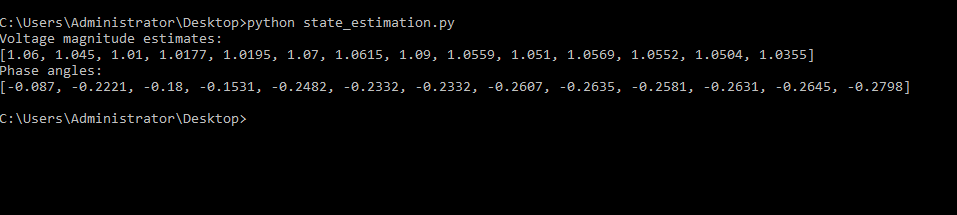
\includegraphics[width=\textwidth]{Figures/state_estimate.png}
\caption{Values of Bus voltages and angles for IEEE 14 Bus system}
\label{fig:se}
\end{figure}

To create an unobservable system, we modify the availability of line flow and bus injection datas, and try finding out the state estimates. We removed the real and reactive power flow measurements in line 6-11 and line 10-11, as well as real and reactive power injection at buses 6,10 and 11. That way, bus 11 is unobservable.
\begin{figure}
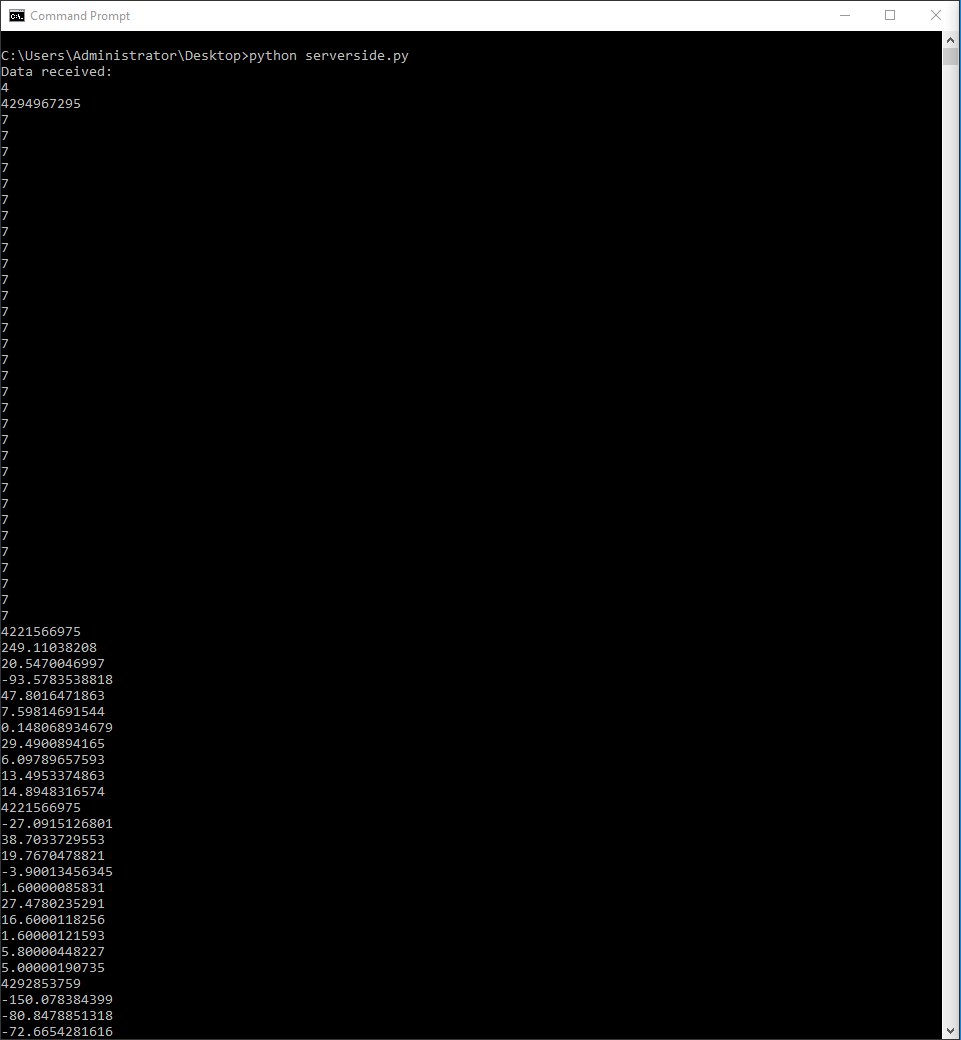
\includegraphics[width=\textwidth]{Figures/unobs_1.png}
\caption{Removing measurements of flows at lines 6-11 and 10-11 and injections at 6,10,11. Part 1}
\label{fig:unobs1}
\end{figure}
\begin{figure}
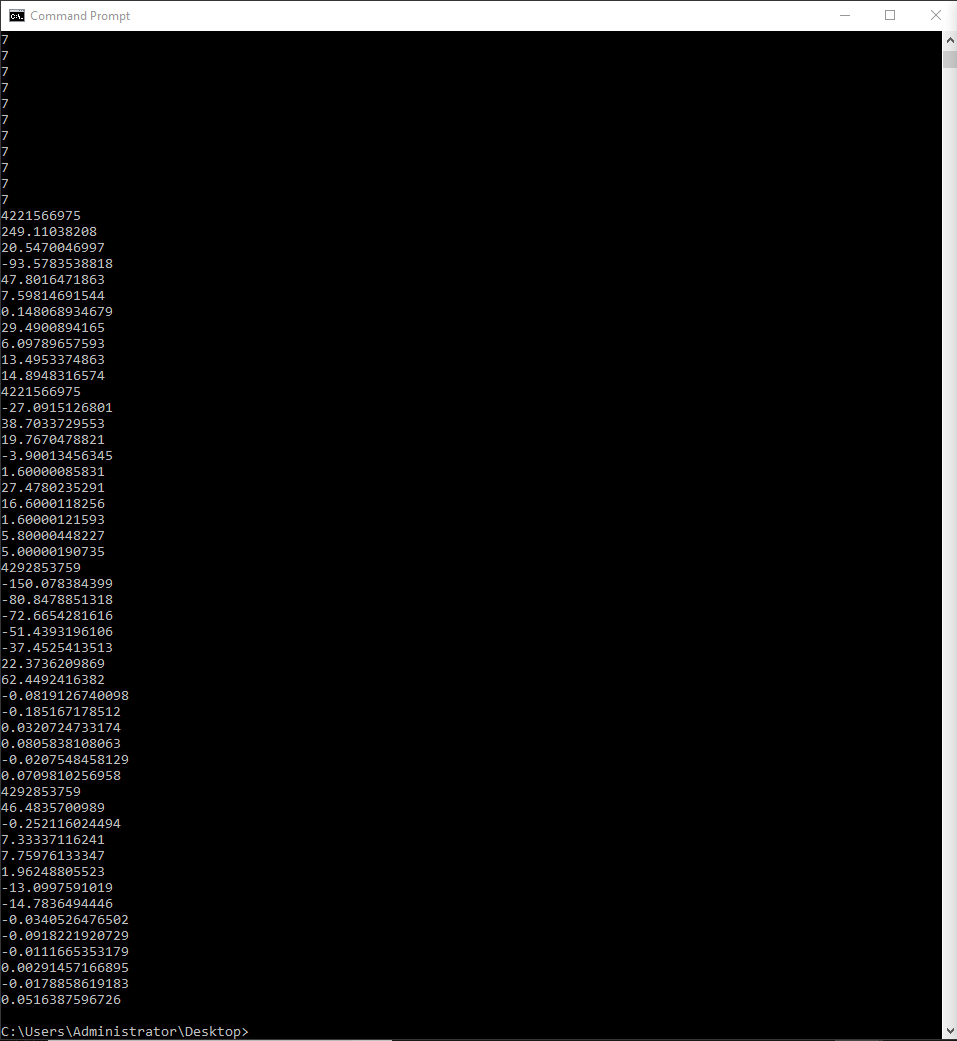
\includegraphics[width=\textwidth]{Figures/unobs_2.png}
\caption{Removing measurements of flows at lines 6-11 and 10-11 and injections at 6,10,11. Part 2}
\label{fig:unobs1}
\end{figure}
\begin{figure}
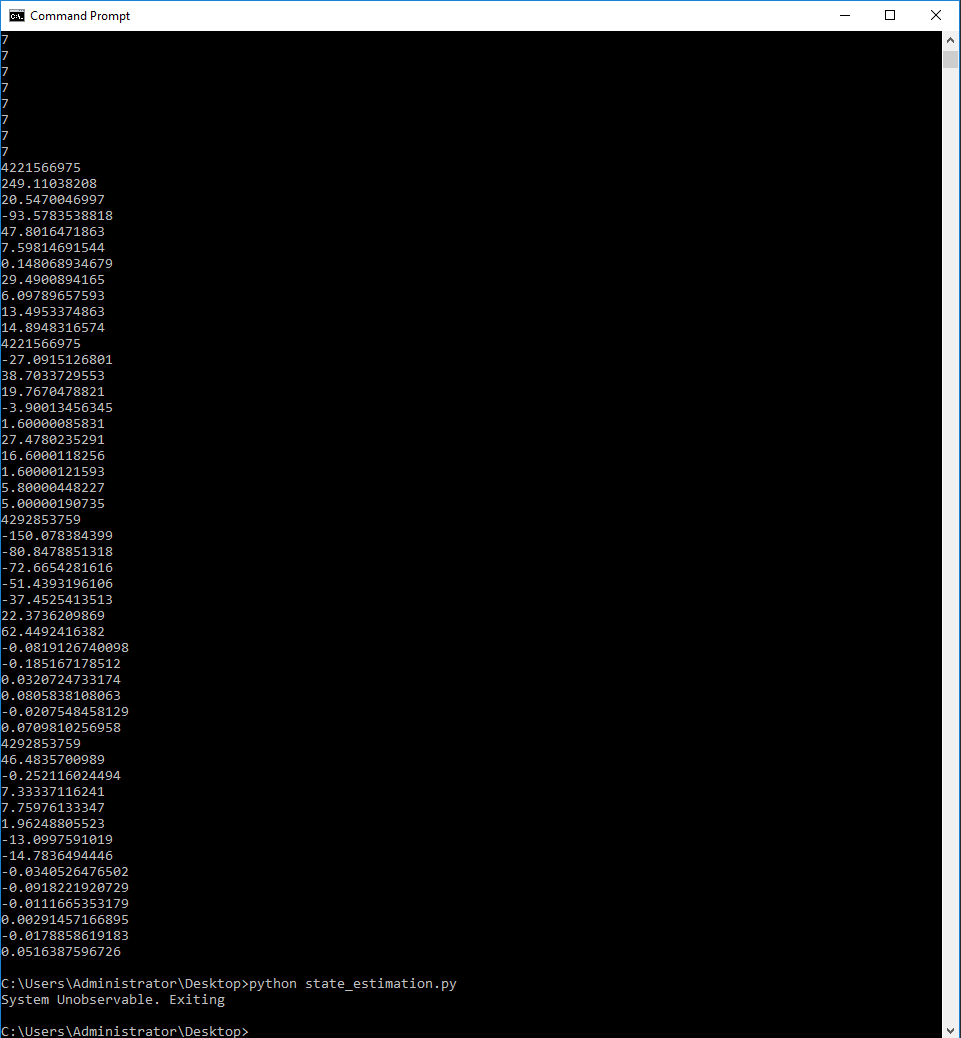
\includegraphics[width=\textwidth]{Figures/non_obs.png}
\caption{Running state estimation with less than neccessary measurements}
\label{fig:unobs1}
\end{figure}


\chapter{Conclusion}

\lipsum[2]

\bibliographystyle{plain}
\bibliography{biblio}

\appendix
\chapter{Appendix}
\section{Server Script to collect data from RTDS and Process it}
\begin{lstlisting}[language=python]
def get_data_from_rtds(self):
		s = socket.socket(socket.AF_INET, socket.SOCK_STREAM)
		s.bind(('', self.port))
		self.rtds_data=[]
		while True:
			data, addr = s.recvfrom(BUFFER_SIZE)
			if len(data) != 0:
				values=data[i:i+4] for i in range(0,len(data),4)
				for value_ascii_str in values:
					value_hex_str = bin(int(binascii.hexillify(value_ascii_str),16))
					f=int(value_hex_str,2)
					self.rtds_data.add(struct.unpack('f',struct.pack('I',f))[0])
				break
\end{lstlisting}

\end{document}
	